%\documentclass[a4paper,11pt]{book}
%\usepackage[spanish]{babel} % Para escribir en Espanol normal
%\usepackage[utf8]{inputenc}
%\usepackage[latin1]{inputenc}
%\usepackage{color}
%\usepackage{array}
%\usepackage{amsmath,amssymb}
%\usepackage{float}
%\usepackage{graphicx}
%\usepackage{subfig}
%\usepackage{enumerate}
%\usepackage{hyperref}%para hacer referencias
%\begin{document}

%Portada del Documento
\chapter{LaTeX}
\setlength{\unitlength}{1 cm} %Especificar unidad de trabajo
\thispagestyle{empty}
\begin{picture}(18,10)
\put(2,1){
\includegraphics[width=9cm,height=4cm]{./imagenes2/aplic.png}}
\end{picture}
\begin{center}

\end{center}

% fin de la portada


\newpage

\section{ Introducción}

LaTex es un procesador de texto orientado especialmente a la creación de libroos, documentos cieníficos y técnicos que contengan fórmula. Es de codigo abierto y el modo en que LaTex interpreta los documentos es mediante etiquetas.
  \subsection{ Requisitos}
      \begin{itemize}
          \item Descargar el motor de LaTex que es MiKTeX.
              \url{  http://miktex.org }
            \begin{figure}[htb]
              \centering
                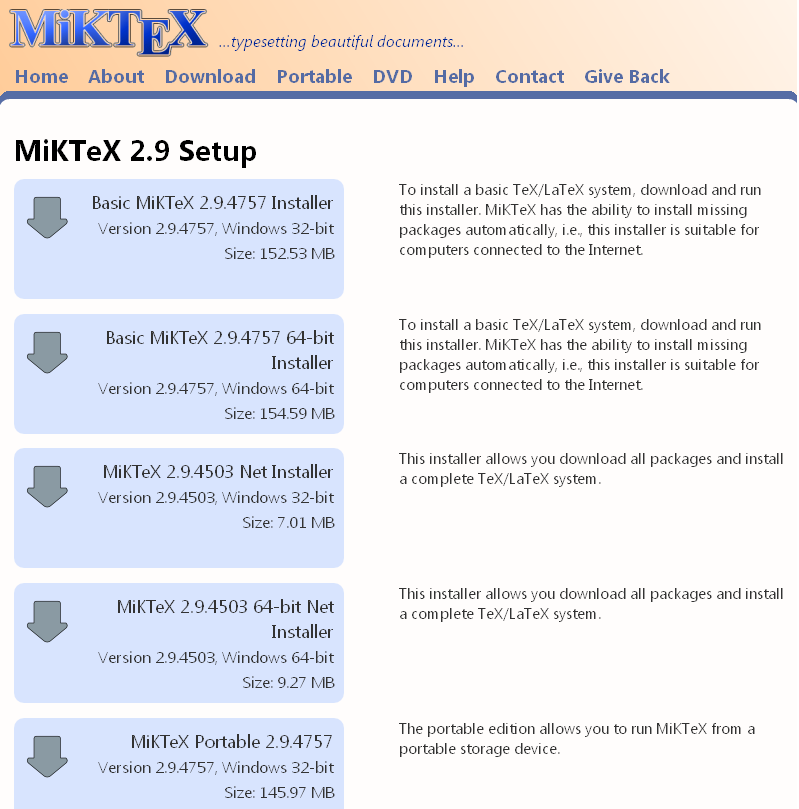
\includegraphics[width=0.58\textwidth]{./imagenes2/image.png}
             \end{figure}

         \item Abrir el area de trabajo que es el TeXworks.
             \begin{figure}[htb]
                \centering
                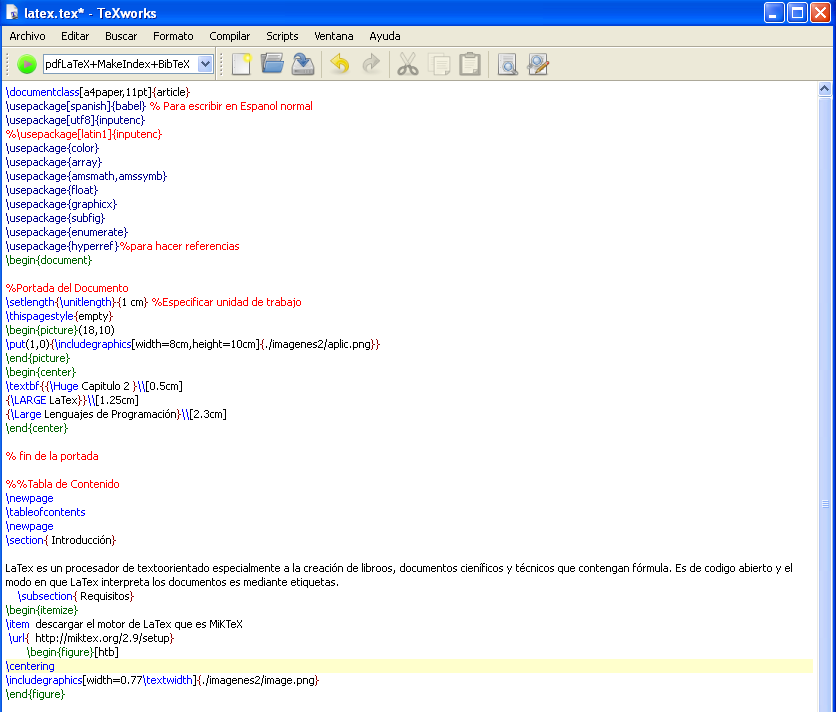
\includegraphics[width=0.57\textwidth]{./imagenes2/image1.png}
             \end{figure}
        \item Compilar.
            \begin{figure}[htb]
               \centering
                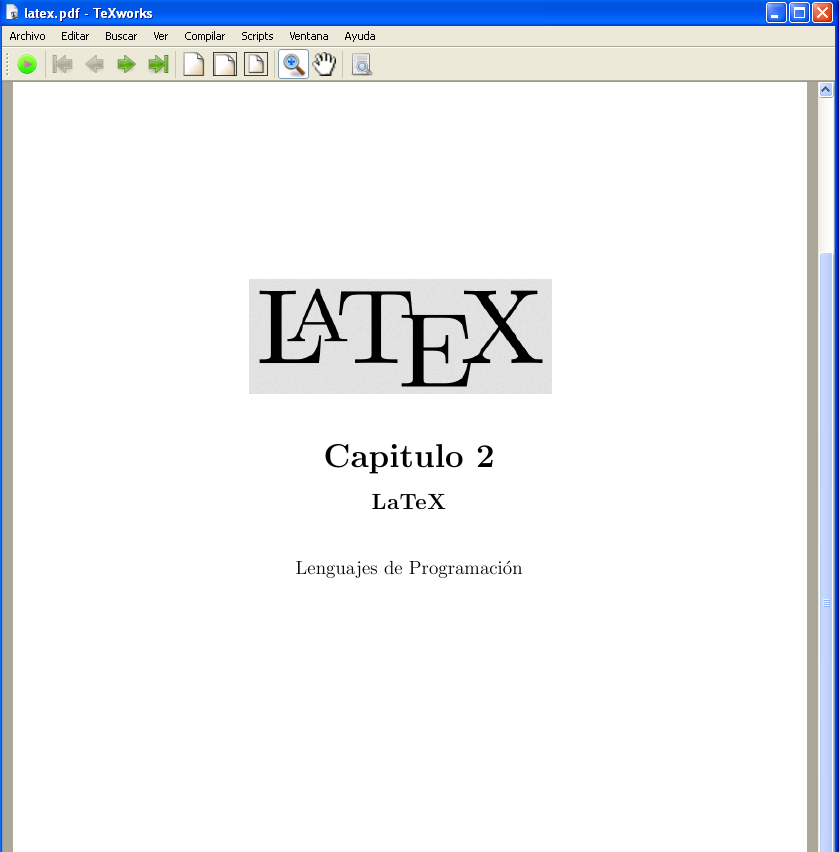
\includegraphics[width=0.58\textwidth]{./imagenes2/image2.png}
             \end{figure}

        \end{itemize}

 \section{ Experiencias}
  \begin{itemize}
\item Al principio me costo mucho trabajar con el codigo de latex para documentar mis proyectos ya que estaba acostumbrada a trabajar con los procesadore de textos habituales como Word.
\item Me rehusaba a usarlo porque me parecia inecesario ya que tenia a Word.
\item Con la ayuda de plantillas comencé a acostumbrarme y puedo decir que ahora lo domino. 
\item Con cada proyecto y presentación que se hizo en el semestre poco a poco he aprendido cosas nuevas.
\item Ahora me he acostumbrado a trabajar mis documentos usando LaTeX y me parece una buena herramienta para desarrollar mi tesis.
\end{itemize}
 \section{ Conclusiones}
  LaTeX es un conjunto de paquetes que permiteformatear textos con calidad tipográfica no es muy complicadosi se esta familiarizado con cualquier lenguaje de marca como HTML  o con un entorno de programacón, muy útil para realizar tesis o reportes de proyectos.

%\end {document}

